% Section 3: The Emergence of Design Paradigm (Revised)
% Target: ~1,500 words

\section{The Emergence of Design Paradigm}
\label{sec:design}

% ===== FIGURE 2: 技术演进时间线 =====
%
% 图表类型: 横向时间线图 (Horizontal timeline diagram)
% 尺寸: 全页宽度 (single-column width)
%
% 【主时间轴】
% 横向时间线: 2018 ──── 2020 ──── 2022 ──── 2024 ──── 2025
%
% 【技术里程碑标注】(在时间轴上下交替标注)
%
% 2018-2019 (预测范式成熟期):
% ┌────────────────────────────────┐
% │ AlphaFold (2018)               │  ↑ Above timeline
% │ CASP13 breakthrough             │
% │ First deep learning structure  │
% └────────────────────────────────┘
%
% 2020-2021 (预测范式突破):
% ┌────────────────────────────────┐  ↓ Below timeline
% │ AlphaFold2 (Jul 2021)          │
% │ "Solving" protein folding      │
% │ Nature publication             │
% └────────────────────────────────┘
% ┌────────────────────────────────┐
% │ RoseTTAFold (2021)             │  ↑ Above
% │ Three-track network            │
% │ Science publication            │
% └────────────────────────────────┘
% ┌────────────────────────────────┐
% │ ESM-1b (2021)                  │  ↓ Below
% │ 650M parameter PLM             │
% │ Language models for proteins   │
% └────────────────────────────────┘
%
% 2022 (设计工具出现):
% ┌────────────────────────────────┐
% │ ProteinMPNN (Sep 2022)         │  ↑ Above
% │ Inverse folding                │
% │ 52.4% sequence recovery        │
% │ Science publication            │
% └────────────────────────────────┘
% ┌────────────────────────────────┐
% │ ESM-2/ESMFold (2022)           │  ↓ Below
% │ 15B parameters                 │
% │ 60× faster than AF2            │
% └────────────────────────────────┘
% ┌────────────────────────────────┐
% │ AlphaFold-Multimer (2022)      │  ↑ Above
% │ Complex prediction             │
% │ 67% interface accuracy         │
% └────────────────────────────────┘
%
% 2023 (生成式设计突破):
% ┌────────────────────────────────┐
% │ RFdiffusion (Feb 2023)         │  ↓ Below
% │ Diffusion for design           │
% │ Cryo-EM validated              │
% │ Nature publication             │
% └────────────────────────────────┘
% ┌────────────────────────────────┐
% │ Chroma (2023)                  │  ↑ Above
% │ Polymer statistics             │
% │ 4000 AA generation             │
% └────────────────────────────────┘
% ┌────────────────────────────────┐
% │ FrameDiff (2023)               │  ↓ Below
% │ SE(3) diffusion                │
% └────────────────────────────────┘
%
% 2024 (高级设计能力):
% ┌────────────────────────────────┐
% │ AlphaFold 3 (May 2024)         │  ↑ Above
% │ Multimodal complexes           │
% │ Diffusion architecture         │
% │ Nature publication             │
% └────────────────────────────────┘
% ┌────────────────────────────────┐
% │ AlphaProteo (Sep 2024)         │  ↓ Below
% │ High-affinity binders          │
% │ 3-300× success rate            │
% │ Nanomolar affinities           │
% └────────────────────────────────┘
% ┌────────────────────────────────┐
% │ RFdiffusionAA (2024)           │  ↑ Above
% │ Small molecule binding         │
% │ Cofactor design                │
% └────────────────────────────────┘
%
% 【阶段分隔线】
% • 2018-2021: "PREDICTION ERA" (蓝色背景区域)
% • 2022-2025: "DESIGN ERA" (绿色背景区域)
% • 在2021-2022之间画粗虚线，标注 "PARADIGM SHIFT"
%
% 【技术类型颜色编码】
% • 结构预测 (蓝色圆点): AlphaFold, RoseTTAFold, ESMFold
% • 语言模型 (紫色圆点): ESM-1b, ESM-2
% • 序列设计 (橙色圆点): ProteinMPNN, ESM-IF1
% • 生成设计 (绿色圆点): RFdiffusion, Chroma, AlphaProteo
%
% 【图例】
% ┌──────────────────────────────────┐
% │ ● 结构预测 (Structure)           │
% │ ● 语言模型 (PLM)                 │
% │ ● 序列设计 (Sequence Design)     │
% │ ● 生成设计 (Generative Design)   │
% └──────────────────────────────────┘
%
% 颜色方案:
% • 时间轴: 深灰色 (#4A4A4A), 粗线 3pt
% • 预测时代背景: 浅蓝色 (#E3F2FD), 透明度30%
% • 设计时代背景: 浅绿色 (#E8F5E9), 透明度30%
% • 分隔线: 红色虚线 (#F44336)
%
% 脚注: "Figure 2: Timeline of major technical breakthroughs in AI-driven protein research (2018-2024). 
%        The paradigm shift from prediction to design occurred around 2021-2022, marked by the emergence 
%        of generative methods capable of creating novel protein sequences and structures."

\begin{figure}[t]
\centering
\resizebox{0.95\textwidth}{!}{%
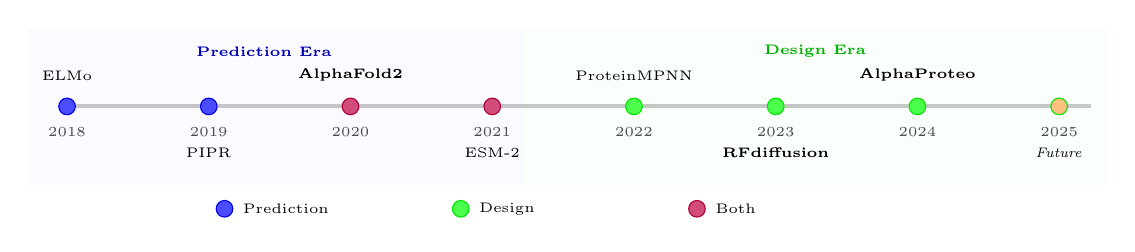
\begin{tikzpicture}[
    milestone/.style={circle, minimum size=6pt, inner sep=0pt},
    predmile/.style={milestone, fill=blue!70, draw=blue!90!black},
    designmile/.style={milestone, fill=green!70, draw=green!90!black},
    bothmile/.style={milestone, fill=purple!70, draw=purple!90!black}
]
% Timeline
\draw[line width=1.5pt, gray!60] (0, 0) -- (13, 0);
% Year markers
\foreach \x/\y in {0/2018, 1.8/2019, 3.6/2020, 5.4/2021, 7.2/2022, 9/2023, 10.8/2024, 12.6/2025} {
    \draw[gray!60] (\x, -0.1) -- (\x, 0.1);
    \node[font=\tiny, below] at (\x, -0.15) {\y};
}
% Phase backgrounds
\fill[blue!5, opacity=0.3] (-0.5, -1) rectangle (5.8, 1);
\fill[green!5, opacity=0.3] (5.8, -1) rectangle (13.2, 1);
\node[font=\tiny\bfseries, blue!70!black] at (2.5, 0.7) {Prediction Era};
\node[font=\tiny\bfseries, green!70!black] at (9.5, 0.7) {Design Era};
% Milestones
\node[predmile] at (0, 0) {};
\node[font=\tiny, above, align=center] at (0, 0.2) {ELMo};
\node[predmile] at (1.8, 0) {};
\node[font=\tiny, below, align=center] at (1.8, -0.4) {PIPR};
\node[bothmile] at (3.6, 0) {};
\node[font=\tiny, above, align=center] at (3.6, 0.2) {\textbf{AlphaFold2}};
\node[bothmile] at (5.4, 0) {};
\node[font=\tiny, below, align=center] at (5.4, -0.4) {ESM-2};
\node[designmile] at (7.2, 0) {};
\node[font=\tiny, above, align=center] at (7.2, 0.2) {ProteinMPNN};
\node[designmile] at (9, 0) {};
\node[font=\tiny, below, align=center] at (9, -0.4) {\textbf{RFdiffusion}};
\node[designmile] at (10.8, 0) {};
\node[font=\tiny, above, align=center] at (10.8, 0.2) {\textbf{AlphaProteo}};
\node[designmile, fill=orange!50] at (12.6, 0) {};
\node[font=\tiny, below, align=center] at (12.6, -0.4) {\textit{Future}};
% Legend
\node[predmile, label=right:{\tiny Prediction}] at (2, -1.3) {};
\node[designmile, label=right:{\tiny Design}] at (5, -1.3) {};
\node[bothmile, label=right:{\tiny Both}] at (8, -1.3) {};
\end{tikzpicture}
}
\caption{Timeline of major technical breakthroughs in AI-driven protein research (2018--2025). The paradigm shift from prediction to design occurred around 2021--2022, marked by the emergence of generative methods capable of creating novel proteins rather than merely analyzing existing ones. \textbf{Milestones shown in bold} (AlphaFold2, RFdiffusion, AlphaProteo) represent transformative advances with extensive experimental validation. \textbf{Color coding:} Blue dots indicate prediction-focused methods that analyze known proteins; green dots indicate design-focused methods that generate novel proteins; purple dots indicate methods spanning both paradigms. The shaded background regions delineate the Prediction Era (2018--2021, characterized by structure prediction breakthroughs) from the Design Era (2022--present, characterized by generative capabilities). The ``Future'' milestone (2025) reflects ongoing development of next-generation systems combining improved accuracy with enhanced computational efficiency.}
\label{fig:timeline}
\end{figure}

In 2021, DeepMind's AlphaFold2 achieved what many considered the ``grand challenge'' of computational biology: predicting protein structures from amino acid sequences with near-experimental accuracy~\citep{jumper2021alphafold}. Just two years later, researchers demonstrated something that would have seemed impossible a decade earlier: designing entirely new proteins that had never existed in nature, validated by cryo-EM structures showing atomic-level agreement with computational models~\citep{watson2023rfdiffusion}. This transition---from predicting what \textit{exists} to creating what \textit{should exist}---represents a fundamental paradigm shift in how artificial intelligence interfaces with protein science.

\subsection{Technical Drivers of the Paradigm Shift}
\label{subsec:drivers}

The emergence of the design paradigm was not a singular event but the convergence of multiple technological breakthroughs occurring between 2021 and 2024: structure prediction advances, generative models for proteins, scaled protein language models, and equivariant neural networks.

\subsubsection{Breakthroughs in Structure Prediction}

AlphaFold2's resolution of the protein folding problem~\citep{jumper2021alphafold} provided the foundation upon which protein design could be built. RoseTTAFold~\citep{baek2021rosettafold}, developed concurrently and published in the same year, demonstrated an alternative three-track architecture that achieved comparable accuracy with different computational trade-offs. The subsequent extension to multimeric complexes through AlphaFold-Multimer~\citep{evans2022alphafoldmultimer} and RoseTTAFold2~\citep{baek2023rosettafold2} expanded the scope to protein-protein interfaces, achieving correct interface prediction for 67\% of heterodimeric complexes. The significance of these advances for design is twofold: structure prediction provides a validation mechanism for designed proteins, and the underlying architectures contain learned representations that can be repurposed for generation. The Invariant Point Attention (IPA) mechanism introduced in AlphaFold2 has become a foundational architectural element in subsequent design systems. AlphaFold 3~\citep{abramson2024alphafold3} extended this capability further to complexes containing proteins, nucleic acids, small molecules, and ions.

\subsubsection{Introduction of Generative Models}

Diffusion models achieved breakthrough performance in image generation before being adapted to the protein domain. The fundamental principle underlying diffusion models is learning to reverse a gradual noising process: given a data distribution (valid protein structures), the forward process progressively adds Gaussian noise until the structure becomes random noise. The reverse process learns to denoise, iteratively recovering structure from noise.

For protein design, the key insight was recognizing that protein backbone conformations can be represented as SE(3) objects---3D structures with rotational and translational symmetries. SE(3) diffusion models~\citep{yim2023se3diffusion} operate directly on the manifold of rigid body frames, where each residue is represented by its position and orientation in 3D space. The denoising network must therefore be equivariant to rotations and translations, maintaining consistency regardless of the coordinate frame. FrameDiff demonstrated this approach could generate diverse, designable protein backbones without relying on pretrained structure prediction networks.

RFdiffusion~\citep{watson2023rfdiffusion} took a different approach by fine-tuning the pretrained RoseTTAFold network as a denoising model. This transfer learning strategy proved highly effective: RoseTTAFold's learned representations of protein structure provided a strong initialization for the generative task, reducing training time and improving sample quality. RFdiffusion conditions generation on partial structures (motifs, functional sites) or target proteins (for binder design), enabling targeted design rather than unconditional generation.

Chroma~\citep{ingraham2023chroma} was designed from the ground up as a generative model with a diffusion process that explicitly respects polymer conformational statistics. By incorporating physical constraints during training, Chroma generates proteins that satisfy both learned statistical patterns and physical plausibility. The system demonstrated generation of proteins up to 4,000 amino acids---far exceeding the typical 100-300 residue range of earlier methods.

An alternative to diffusion is flow matching, which learns deterministic trajectories through the space of protein structures rather than stochastic denoising paths. FoldFlow~\citep{bose2023foldflow} demonstrated that SE(3) flow matching can achieve comparable sample quality to diffusion while potentially offering better computational efficiency and mode coverage. However, flow-based approaches currently lag diffusion models in practical protein design applications, with fewer published experimental validations.

These generative approaches share common advantages: controllable generation through conditioning on specific constraints such as binding sites or symmetry requirements, natural production of diverse candidate structures for design space exploration, and learning the distribution of valid structures directly from data without hand-crafted energy functions. DiffDock-PP~\citep{ketata2023diffdockpp} adapted diffusion to protein-protein docking, treating pose generation as a generative process rather than optimization and achieving 44\% sampling success compared to 8\% for baselines.

\subsubsection{Scaling of Protein Language Models}

Protein language models (PLMs) learn meaningful protein representations through self-supervised pretraining on large sequence databases. ESM-1b~\citep{rives2021esm1b} demonstrated that transformer models capture evolutionary, structural, and functional information from sequence alone. ESM-2~\citep{lin2023esm2}, scaled to 15 billion parameters, achieved atomic-level structure prediction directly from sequence, with ESMFold running 60$\times$ faster than AlphaFold2. ProtTrans~\citep{elnaggar2021prottrans} established that encoder-only models outperform encoder-decoder architectures for protein understanding tasks.

These models provide a learned prior over protein sequences---encoding what sequences are likely to fold into stable, functional proteins. SaProt~\citep{su2024saprot} advanced this by introducing a structure-aware vocabulary that combines amino acid tokens with structural tokens. MINT~\citep{ullanat2025mint} and PLM-interact~\citep{zhao2025plminteract} extended PLMs specifically for PPI tasks, training on protein sets to model interaction propensities contextually.

\subsubsection{Development of Equivariant Neural Networks}

Equivariant neural networks process 3D geometric data while respecting physical symmetries, addressing the challenge that protein function depends on 3D structure but the same structure can be represented in any rotated or translated coordinate frame. This property is critical for protein design: a generated protein's validity should not depend on the arbitrary coordinate system in which it was generated.

SE(3)-Transformers~\citep{fuchs2020se3transformer} introduced attention mechanisms equivariant to 3D rotations and translations. The key architectural innovation is ensuring that attention weights depend only on relative positions and orientations---quantities invariant to global rotations---while the output features transform appropriately under coordinate changes. This equivariance-by-construction eliminates the need for data augmentation to cover all possible orientations, improving sample efficiency and generalization.

Geometric Vector Perceptrons (GVPs)~\citep{jing2021gvp} provided a simpler but equally effective approach through scalar-vector separation. Each node in the protein graph maintains both scalar features (amino acid type, biochemical properties) and vector features (spatial orientations, directional interactions). Message passing operates on both: scalar messages aggregate through standard attention or summation, while vector messages aggregate through rotation-equivariant operations. GVP-GNNs achieved state-of-the-art performance on structure-based tasks while maintaining computational efficiency suitable for design workflows.

AlphaFold2's Invariant Point Attention (IPA)~\citep{jumper2021alphafold} represents a third approach: rather than enforcing equivariance through architectural constraints, IPA projects 3D coordinates onto a learned frame where attention operations become rotation-invariant. Each residue maintains a local coordinate frame, and attention operates on the relative positions within these frames. This design choice has been widely adopted in subsequent structure prediction and design systems, including RFdiffusion.

Recent work has extended these geometric approaches to protein interface prediction. ScanNet~\citep{tubiana2022scannet} combined geometric deep learning with spatial attention for interpretable binding site prediction. PeSTo~\citep{krapp2023pesto} achieved parameter-free geometric prediction of protein binding interfaces, enabling rapid scanning of the growing ``foldome'' of predicted structures. GeoPLM~\citep{zhang2023geoplm} integrated geometric structure pretraining with protein language models, learning representations that capture both sequence patterns and spatial relationships.

These architectures provide three key benefits for protein design: guaranteeing physical consistency regardless of coordinate frame, improving sample efficiency by encoding geometric relationships by construction, and enabling better generalization to novel structures that differ from training examples.

\subsection{Milestone Works in the Design Era}
\label{subsec:milestones}

The convergence of these technical drivers has produced breakthrough works organized by primary function: backbone generation, sequence design, and binder design (Table~\ref{tab:design_tools}).

% ===== TABLE 2: 主流设计工具对比 =====
%
% 表格类型: 多列对比表 (Multi-column comparison table)
% 宽度: 全页宽度 (full-width)
%
% 表头设计:
% ┌─────────────────────────────────────────────────────────────────────────────────────────┐
% │ Method       │ Year │ Input               │ Output        │ Success Rate │ Validation │
% ├─────────────────────────────────────────────────────────────────────────────────────────┤
%
% 【数据行】
%
% Row 1: RFdiffusion
% │ RFdiffusion  │ 2023 │ • Target structure  │ • Backbone    │ 10-50%       │ • Cryo-EM  │
% │              │      │ • Symmetry specs    │ • Sequence    │ (binding)    │   (100s)   │
% │              │      │ • Motif constraints │   candidates  │              │ • X-ray    │
% │              │      │                     │               │              │   (10s)    │
%
% Row 2: AlphaProteo
% │ AlphaProteo  │ 2024 │ • Target structure  │ • Binder      │ 3-300×       │ • SPR      │
% │              │      │ • Binding site      │   structures  │   vs         │   (affinity│
% │              │      │   (optional)        │ • Sequences   │   baseline   │   KD: nM)  │
% │              │      │                     │               │              │ • BLI      │
% │              │      │                     │               │              │ • Flow     │
% │              │      │                     │               │              │   cytometry│
%
% Row 3: ProteinMPNN
% │ ProteinMPNN  │ 2022 │ • Backbone          │ • Sequences   │ 52.4%        │ • X-ray    │
% │              │      │   structure         │   (multiple)  │ (native      │   (seq     │
% │              │      │ • Multi-chain       │               │ recovery)    │   recovery)│
% │              │      │   specification     │               │              │ • Stability│
% │              │      │                     │               │              │   assays   │
%
% Row 4: ESM-IF1
% │ ESM-IF1      │ 2022 │ • Backbone          │ • Sequences   │ 51%          │ • In silico│
% │              │      │   structure         │ • ΔΔG         │ (native      │   validation│
% │              │      │                     │   predictions │ recovery)    │ • 12M      │
% │              │      │                     │               │              │   training │
% │              │      │                     │               │              │   structures│
%
% Row 5: Chroma
% │ Chroma       │ 2023 │ • Size constraints  │ • Full        │ 70-90%       │ • MD       │
% │              │      │ • Property specs    │   proteins    │ (designability│   simulation│
% │              │      │   (optional)        │   (up to      │ score)       │ • In silico│
% │              │      │                     │   4000 AA)    │              │   foldability│
%
% Row 6: DiffDock-PP
% │ DiffDock-PP  │ 2023 │ • Two protein       │ • Docked      │ 44%          │ • Benchmark│
% │              │      │   structures        │   poses       │ (top-10      │   (DBD5)   │
% │              │      │                     │   (ranked)    │   success)   │ • vs       │
% │              │      │                     │               │              │   8%       │
% │              │      │                     │               │              │   baseline │
%
% Row 7: RFdiffusionAA
% │ RFdiffusionAA│ 2024 │ • Target structure  │ • Binding     │ Not reported │ • Biochemical│
% │              │      │ • Small molecule    │   pockets     │ (early      │   assays   │
% │              │      │   structure         │ • Sequences   │ stage)       │ • Heme     │
% │              │      │                     │               │              │   binding  │
%
% 【表格宽度调整建议】
% • 使用 \small 或 \footnotesize 字体
% • 列宽分配: Method(2cm), Year(0.8cm), Input(2.5cm), Output(2cm), Success(2cm), Validation(2cm)
% • 如空间不足，可将"Validation"和"Success Rate"合并为"Performance & Validation"
%
% 【特殊格式】
% • RFdiffusion, AlphaProteo: 加粗（代表性方法）
% • Success Rate列: 对高成功率使用绿色背景
% • Year列: 按时间排序
%
% 【脚注】
% 表格下方添加注释:
% † Success rates vary by target difficulty; ranges reflect published data across multiple targets.
% ‡ Validation methods include experimental (Cryo-EM, X-ray, SPR, BLI) and computational metrics.
%
% 颜色方案:
% • 表头: 浅灰色背景 (#F5F5F5)
% • 重点方法行(RFdiffusion, AlphaProteo): 浅绿色背景 (#E8F5E9)
% • 其他行: 白色背景交替 (#FFFFFF, #FAFAFA)

\begin{table}[h]
\centering
\caption{Comparison of major AI-driven protein design tools (2022-2024)}
\label{tab:design_tools}
\small
\begin{adjustbox}{max width=\textwidth}
\begin{tabular}{@{}llllll@{}}
\toprule
\textbf{Method} & \textbf{Year} & \textbf{Input} & \textbf{Output} & \textbf{Success Rate}$^\dagger$ & \textbf{Validation}$^\ddagger$ \\
\midrule
\textbf{RFdiffusion} & 2023 & Target structure, & Backbone, & 10--50\% & Cryo-EM (100s), \\
& & symmetry, motifs & sequences & (binding) & X-ray (10s) \\
\addlinespace
\textbf{AlphaProteo} & 2024 & Target structure, & Binder & 3--300$\times$ & SPR/BLI, \\
& & binding site & structures & vs baseline & KD: nM range \\
\addlinespace
ProteinMPNN & 2022 & Backbone structure & Sequences & 52.4\% & X-ray, stability \\
& & (multi-chain) & (multiple) & (recovery) & assays \\
\addlinespace
ESM-IF1 & 2022 & Backbone structure & Sequences, & 51\% & In silico, \\
& & & $\Delta\Delta G$ & (recovery) & 12M structures \\
\addlinespace
Chroma & 2023 & Size, properties & Full proteins & 70--90\% & MD simulation, \\
& & (optional) & (to 4000 AA) & (designability) & foldability \\
\addlinespace
DiffDock-PP & 2023 & Two structures & Docked poses & 44\% & Benchmark \\
& & & (ranked) & (top-10) & (vs 8\% baseline) \\
\bottomrule
\end{tabular}
\end{adjustbox}
\begin{flushleft}
\footnotesize{$^\dagger$Success rates vary by target difficulty; ranges reflect published data across multiple targets.}\\
\footnotesize{$^\ddagger$Validation methods include experimental (Cryo-EM, X-ray, SPR, BLI) and computational metrics.}\\
\footnotesize{$^\S$Computational requirements: RFdiffusion (16--32GB GPU, $\sim$2--5 min/100 residues), AlphaProteo (proprietary),}\\
\footnotesize{\hspace{2.3cm}ProteinMPNN ($<$4GB/CPU-capable, $\sim$1--2 s/100 residues), ESM-IF1 (8GB), Chroma (24GB+), DiffDock-PP (8GB).}\\
\footnotesize{\hspace{2.3cm}Training costs: ESM-2 required hundreds of GPU-years. Inference times measured on single GPU/CPU.}
\end{flushleft}
\end{table}

\subsubsection{Backbone Generation: RFdiffusion and Chroma}

RFdiffusion~\citep{watson2023rfdiffusion} fine-tuned the RoseTTAFold structure prediction network on protein structure denoising tasks. Starting from RoseTTAFold's pretrained weights, the model learned the reverse diffusion process through a carefully designed training curriculum: initial training on single-domain proteins, followed by fine-tuning on protein complexes and conditional generation tasks. 

Key innovations include leveraging pretrained representations to reduce training time from months to weeks, conditioning on partial structures through inpainting for targeted design (preserving functional motifs while designing surrounding scaffolds), and enabling de novo binder design through target structure conditioning where the diffusion process generates binders complementary to the target's binding site.

Experimental validation demonstrated remarkable success: across multiple target proteins including SARS-CoV-2 spike, influenza hemagglutinin, and PD-1, RFdiffusion-generated binders showed expression rates of 70--90\% and binding success rates of 10--50\% depending on target difficulty. Cryo-EM structures of designed binders confirmed atomic-level agreement with computational models, with backbone RMSD values of 0.5--1.5 \AA{} for successful designs. However, success rates vary dramatically by target: well-structured proteins with deep binding pockets achieve higher success rates than flat, featureless surfaces.

Chroma~\citep{ingraham2023chroma} took a different approach, designed from the ground up as a generative model with a diffusion process that explicitly respects polymer conformational statistics. The key architectural innovation is incorporating physical constraints directly into the generative process: bond lengths, bond angles, and dihedral preferences are encoded in the model's prior, ensuring generated structures are physically plausible. Chroma demonstrated generation of proteins up to 4,000 amino acids---far exceeding the typical 100-300 residue range of earlier methods---and introduced conditional generation through classifier-free guidance, enabling design for specific properties including stability, solubility, and binding affinity.

\subsubsection{Sequence Design: ProteinMPNN and ESM-IF1}

Given a backbone structure, the inverse folding problem asks what sequence will fold into that structure. ProteinMPNN~\citep{dauparas2022proteinmpnn} uses message passing neural networks to process backbone geometry and generate sequences, achieving 52.4\% native sequence recovery on native backbones. It supports multi-chain design of protein-protein interfaces in a single forward pass and generates sequences in milliseconds for high-throughput design. ESM-IF1~\citep{hsu2022esmif1} provides an alternative using sequence-to-sequence transformers trained on 12 million AlphaFold2-predicted structures, achieving 51\% native sequence recovery while also predicting protein stability changes upon mutation.

\subsubsection{Binder Design: AlphaProteo}

AlphaProteo~\citep{zambaldi2024alphaproteo} represents the most advanced demonstration of AI-driven protein binder design to date. Given a target protein structure, it generates sequences and structures of proteins designed to bind with high affinity through an integrated pipeline combining: (1) target structure analysis to identify favorable binding regions; (2) binding site prediction leveraging advances in deep learning~\citep{zeng2020binding}; (3) backbone generation conditioned on the target binding site; (4) sequence design for structural stability and interface complementarity; and (5) computational affinity screening to prioritize candidates.

The experimental results are striking. Across seven diverse protein targets---including viral proteins (SARS-CoV-2 spike, VEGF-A), cytokines (IL-7), and immune checkpoint proteins (PD-L1, CTLA-4)---AlphaProteo achieved binding success rates 3--300$\times$ higher than RFdiffusion-based approaches. Multiple designed binders achieved nanomolar affinities (K$_D$ = 1--100 nM) without any experimental optimization through directed evolution or affinity maturation. For comparison, typical antibody therapeutics require extensive optimization to reach this affinity range.

The technical innovations include conditioning the generative model on predicted binding energy landscapes rather than just structural geometry, incorporating evolutionary constraints from multiple sequence alignments of natural binders where available, and using ensemble predictions from multiple models to estimate uncertainty and filter low-confidence designs. However, limitations remain: AlphaProteo showed poor performance on targets with shallow binding surfaces, and designs for some targets failed to express in standard expression systems despite computational predictions of stability.

\subsubsection{Multi-Modal Prediction: AlphaFold 3 and RoseTTAFold All-Atom}

AlphaFold 3~\citep{abramson2024alphafold3} replaced AlphaFold2's structure module with a diffusion model, enabling prediction of complexes containing proteins, DNA, RNA, small molecules, and ions. RoseTTAFold All-Atom~\citep{krishna2024rfaa} similarly extends RoseTTAFold to full biological assemblies and introduces RFdiffusionAA for de novo design of protein binding pockets around small molecules, with experimentally validated designs for heme and bilin binding proteins. These systems provide high-quality predictions of possible interactions, computational verification of designed complex structures, and extension to design of proteins interacting with non-protein partners.

\subsection{The Relationship Between Prediction and Design}
\label{subsec:relationship}

Prediction and design are not opposing paradigms but complementary capabilities that reinforce each other in three ways.

\textbf{Prediction as Foundation.} Every design system relies on prediction capabilities. RFdiffusion was initialized from RoseTTAFold's pretrained weights. ProteinMPNN is trained to predict sequences that fold into given structures. AlphaProteo uses structure prediction for validation and filtering. The knowledge embedded in prediction models provides the prior that makes design tractable.

\textbf{Design as Iterative Prediction.} The design process can be viewed as a series of predictions: structure prediction of the target, interface prediction for favorable binding sites, backbone generation as inverse structure prediction, sequence design for backbone compatibility, complex prediction of the binder-target pair, and affinity prediction of the designed interaction. Each step involves prediction, and design succeeds when all predictions align.

\textbf{Verification Through Prediction.} Prediction provides the verification mechanism for designed proteins. Before experimental validation, designed structures can be computationally folded to verify structural integrity, with pLDDT $>$ 90 commonly used as a threshold. This computational verification dramatically reduces experimental burden: researchers can computationally filter thousands of candidates to tens of high-confidence designs.

The relationship is bidirectional: design also advances prediction by providing test cases that explore novel regions of sequence-structure space not represented in natural proteins, revealing limitations that drive prediction method improvement.

\subsection{Critical Assessment: Successes and Limitations}
\label{subsec:critical}

While the design paradigm has achieved remarkable successes, a balanced assessment requires examining both achievements and limitations.

\subsubsection{Success Rate Variability}

Reported success rates vary dramatically across studies, targets, and success criteria. RFdiffusion reported 10--50\% success rates for binder design~\citep{watson2023rfdiffusion}, while AlphaProteo achieved 3--300$\times$ improvement over baselines~\citep{zambaldi2024alphaproteo}. However, these numbers are not directly comparable: studies use different definitions of ``success'' (binding in any affinity range vs. nanomolar affinity), different experimental protocols (yeast display vs. mammalian expression), and different target difficulty levels (well-characterized proteins vs. challenging targets).

Analysis of published data reveals consistent patterns: success rates are highest for targets with deep, well-defined binding pockets (enzyme active sites, cytokine-receptor interfaces), intermediate for targets with shallow but accessible surfaces (protein-protein interaction interfaces), and lowest for targets with flat, featureless surfaces or high flexibility. This gradient suggests that current methods excel at optimizing shape complementarity but struggle with the more subtle chemical features required for challenging targets.

\vspace{0.5em}
\noindent
\textbf{Note on Success Rate Comparisons:} Direct comparison of success rates across methods is complicated by methodological differences. AlphaProteo's reported ``3--300$\times$ improvement'' refers to relative success rate compared to RFdiffusion baseline on the same targets, not absolute success percentages. RFdiffusion's ``10--50\%'' represents absolute binding success rates across diverse targets. The two metrics are therefore not directly comparable, and cross-method comparisons should be interpreted with caution.

\subsubsection{Failure Modes}

Several systematic failure modes have been identified: (1) \textit{Expression failure}: 10--30\% of computationally validated designs fail to express in standard systems, often due to aggregation propensity or protease susceptibility not captured by structural metrics; Bennett et al.~\citep{bennett2025low} reported that binders for many targets failed due to low expression, nonspecific binding, or undetectable affinity despite successful computational validation; (2) \textit{Misfolding}: despite high pLDDT scores from structure prediction, some designs populate alternative conformations in solution, suggesting that current computational validation may not capture the full conformational ensemble---recent work by Rao et al.~\citep{rao2026adversarial} demonstrated that adversarial sequence mutations can produce non-physical structures that AlphaFold nevertheless predicts with high confidence; (3) \textit{Off-target binding}: designs selected for high affinity to the target may also bind related proteins, limiting specificity---a particular concern for therapeutic applications where selectivity is critical; (4) \textit{Stability-affinity tradeoffs}: mutations that improve affinity often destabilize the scaffold, requiring multi-objective optimization not fully addressed by current pipelines. A systematic study by Chu et al.~\citep{chu2025prediction} found that roughly half of designed proteins failed at various experimental stages, with many failed designs having better computational confidence metrics than successful designs, highlighting the limitations of current predictive metrics.

\subsubsection{Comparison with Traditional Approaches}

AI-driven design shows clear advantages over traditional computational design in throughput (hours vs. months), success rates for challenging targets (particularly those lacking natural templates), and the ability to explore novel fold topologies. However, traditional approaches---particularly those incorporating extensive experimental screening and directed evolution---remain competitive for well-characterized protein families where evolution can optimize beyond current computational energy functions. The highest-affinity binders often result from hybrid approaches: computational design provides starting points, and directed evolution refines affinity and developability.

\subsubsection{The Hallucination Problem}

A fundamental challenge in generative protein design is distinguishing genuine design from ``hallucination''---the generation of structures that appear protein-like to computational metrics but lack physical plausibility~\citep{anishchenko2021hallucination}. Deep network hallucination, first demonstrated by Anishchenko et al., showed that neural networks trained on protein structures can generate novel backbones that score well on computational metrics but may or may not correspond to foldable sequences.

This problem manifests in several ways: (1) \textit{Backbone incoherence}: Generated backbone geometries may violate Ramachandran constraints or create steric clashes that are not detected by coarse-grained validation; (2) \textit{Sequence-structure mismatch}: The inverse folding problem has multiple solutions, and generated sequences may not actually fold into the designed structure; (3) \textit{Energy landscape pathology}: Designed proteins may have native-like lowest-energy states but high-energy barriers or competing minima that prevent folding in practice.

Current approaches mitigate hallucination through iterative validation: structure prediction on generated sequences, molecular dynamics simulation to assess stability, and increasingly, experimental characterization. However, the hallucination problem underscores that computational metrics---however sophisticated---cannot fully substitute for physical reality. The most reliable designs result from pipelines that combine computational generation with multiple validation stages.

\vspace{0.5em}
\noindent
\textbf{Limitations of Structural Validation.} Even experimental validation by cryo-EM and X-ray crystallography has important caveats. These methods capture static snapshots at crystalline or vitrified conditions that may not reflect dynamic behavior in solution. Cryo-EM averages over millions of particles and potentially obscuring rare conformations or conformational heterogeneity. X-ray crystallography selects for crystallizable conformations that may differ from the solution state. Neither technique directly captures protein dynamics, solution behavior, or thermodynamic stability under physiological conditions. These limitations suggest that comprehensive validation requires multiple complementary approaches: biophysical characterization (SPR, ITC, BLI for affinity), solution scattering (SAXS, DLS) for oligomeric state), and increasingly, NMR for dynamic information.

\vspace{0.5em}
\noindent
\textbf{Limitations of Structural Validation.} Experimental validation by cryo-EM and X-ray crystallography provides atomic-level confirmation of designed structures, but these methods have inherent limitations. Cryo-EM captures static snapshots of protein conformations and may miss dynamic or transient states~\citep{kleywegt2023validation}. X-ray crystallography selects for conformations that crystallize, which may not represent the dominant species in solution. Neither method fully captures conformational dynamics, allosteric effects, or in-solution behavior. A design that appears correct by structural methods may still exhibit unexpected behavior in functional assays, underscoring the importance of complementary biochemical and biophysical characterization beyond structural validation alone.

The paradigm shift is therefore not a complete replacement of traditional methods but rather a fundamental expansion of what is tractable. Design targets that were previously infeasible---novel scaffolds, de novo interfaces, proteins binding to challenging targets---are now accessible, while established methods continue to excel in their domains of strength.

\vspace{1em}
\noindent
The technical drivers, milestone works, and critical assessment described in this section establish the foundation for the design paradigm. The following sections examine the specific tasks enabled by these capabilities (Section~\ref{sec:design_tasks}) and the technologies underlying them (Section~\ref{sec:technologies}).
